\documentclass[longdoc,bigchapter, colorback,accentcolor=tud1c,12pt,numbersubsubsec]{tudreport}

\usepackage{hyperref}
\usepackage{subfigure}
\usepackage{epstopdf}
\usepackage[]{acronym}
\usepackage[utf8]{inputenc}
\usepackage[ngerman]{babel}


\usepackage{subfigure}


\usepackage{geometry}
\geometry{a4paper,left=25mm,right=20mm, top=1.5cm, bottom=1.5cm}
\usepackage{mathdesign}
\usepackage[]{subfigure}
\usepackage[]{graphicx}
%\usepackage[]{natbib}
\usepackage[]{amsmath}
%\usepackage{dsfont}
\usepackage{color}
\usepackage{booktabs}
\usepackage{verbatim}
\usepackage{listings}
\usepackage[ruled,chapter]{algorithm}
\usepackage[]{algorithmic}

\definecolor{red}{rgb}{1.,0.,0.}
%Eigene Befehle
\newcommand{\todo}{\textcolor{red}{\textbf{ToDo}}}
\newcommand{\image}{\textcolor{red}{\textbf{\\insert Image\\}}}
\newcommand{\quelle}{\textcolor{red}{\textbf{Quellenangabe}}}
\newcommand{\link}{\textcolor{red}{\textbf{Link}}}
\newcommand{\formel}{\textcolor{red}{\textbf{\\Formel\\}}}
\newcommand{\tabelle}{\textcolor{red}{\textbf{\\Tabelle\\}}}
% Pfad entlang dem die Bilder gesucht werden.
\graphicspath{{bilder/}}
%Kopfzeile
\linespread{1.2}                                 % Zeilenabstand
\setlength{\parindent}{6mm}                      % Absatzeinzug

\title{Sensitivität numerischer Vorhersagen des Wirkungsgrads von Hochdruckturbinen}
\subtitle{ADP | Keijo Buss, Dominik Henzel, Markus Degenhardt, Simon Lippert }
\subsubtitle{Betreuer: Faramarz Bakhtiari, Marius Schneider | Prof.Dr.-Ing.H.-P. Schiffer}
\institution{Fachbereich Maschinenbau\\Institut für Gasturbinen,\\ Luft- und Raumfahrtantriebe}
%Hier wird entweder ein Text für das Institut angewählt oder ein Logo
%\institution{Fachgebiet fŸr \\Numerische Berechnungsverfahren \\im Maschinenbau}
%\setinstitutionlogo[height]{CE}

%%% Untere Titelrückseite
\lowertitleback{%
	Keijo Buss, Dominik Henzel, Markus Degenhardt, Simon Lippert\\
	Studiengang: Computational Engineering M.Sc.\\ \\
	Thema: Sensitivität numerischer Vorhersagen des Wirkungsgrads von Hochdruckturbinen\\\\
	Eingereicht: \today\\ \\
	%Rahmeninformationen
	Betreuer: Faramarz Bakhtiari\\
	\hspace*{4em} Marius Schneider\\\\
	Prof.Dr.-Ing.H.-P. Schiffer \\
	Fachgebiet Gasturbinen, Luft- und Raumfahrtantriebe\\
	Technische Universität Darmstadt\\
	Otto-Berndt-Straße 2\\
	64287 Darmstadt}
% %%%%%%%%%%%%%%%%%%% Hier beginnt das Dokument
\begin{document}
	\maketitle
	% Verzeichnisse mit römischen Seitenzahlen
	\cleardoublepage
	\pagenumbering{roman}
	\addcontentsline{toc}{chapter}{Abstract}
	%******  Abstract **************

\begin{abstract}
%\setlength{\baselineskip}{11pt}
Die Zuverlässigkeit numerischer Vorhersagen des Wirkungsgrades von Turbinenstufen ist ein wichtiger Bestandteil diverser Forschungsaktivitäten wie Parameterstudien und Optimierungen. Mit zunehmender Komplexität der numerischen Modelle und der simulierten physikalischen Phänomene nimmt jedoch auch die Fehleranfälligkeit der numerischen Vorhersagen zu. Für eine sinnvolle Interpretation der numerischen Ergebnisse ist die Kenntnis der Einflussgrößen daher sehr wichtig. Um die eben genannte numerische Fehleranfälligkeit genauer zu untersuchen, werden zwei Testfälle herangezogen. Zum einen wird eine 1,5 stufige Aachenturbine simuliert, zum anderen werden die Verbindungsstellen einzelner Domänen, sogenannte Interfaces, in einem einfachen Modell eines zweigeteilten Kanals untersucht. Zunächst erfolgt eine Gitterstudie der zu untersuchenden Aachenturbine, gefolgt von der Untersuchung von Einflussfaktoren auf den Wirkungsgrad.

\end{abstract}
	\section*{Erklärung}

Hiermit versichere ich, die vorliegende Bachelorarbeit ohne Hilfe Dritter nur mit den angegebenen Quellen und Hilfsmitteln angefertigt zu haben. Alle Stellen, die den Quellen entnommen wurden, sind als solche kenntlich gemacht worden. Ich bin mir bewusst, dass bei Abgabe einer falschen Erklärung die Arbeit als nicht bestanden gewertet wird. \\ \\

Darmstadt, den \today

%\vspace*{130mm}
%%\hspace*{70mm}
%\begin{minipage}{129.5mm}
%
 % Hiermit versichere ich, die vorliegende Arbeit unter der
 % Betreuung von Prof.~Dr.~X.~Xxxxxx und Dxxx.-Ing.~X.~Xxxxx 
%  nur mit den angegebenen Hilfsmitteln selbst"andig angefertigt
 % zu haben. \\ [20mm]
%
%Darmstadt, den \date{\today}
%
%\end{minipage}
%\renewcommand{\thepage}{\arabic{page}}
%\setcounter{page}{1}
%\newpage

%%% Local Variables: 
%%% mode: latex
%%% TeX-master: "main"
%%% End: 


 
	\tableofcontents

	
	% Eigentlicher Text mit arabischen Seitenzahlen
	\cleardoublepage
	\pagenumbering{arabic}
	\setcounter{page}{1}
	%Einbinden der einzelnen Kapitel
	%\chapter{Beispiele}
Test

\section{Beispielabbildung}
\begin{figure}
	\centering
	\label{simaufbau}
	\includegraphics[width=0.7\textwidth,angle=90]{screen.eps}
	\caption{Anordnung des umströmten Zylinders}
\end{figure}

\section{Beispieltabelle}
Beispieltabelle \ref{simaufbaufreqs}

\begin{table}[H]
	\caption{Unterschiedliche Frequenzen des oszillierenden Zylinders}
	\centering
	\begin{tabular}{l l l l}
		\hline
		Fall&$Y_0/d$&$f_0 d/U_0$& $f_0$\\ \hline
		M1 & 0,3 & 0,14& $2,205\text{Hz}$\\
		M2 & 0,3 & 0,17& $2,677\text{Hz}$\\
		M3 & 0,3 & 0,19& $2,992\text{Hz}$\\
		M4 & 0,3 & 0,21& $3,307\text{Hz}$\\
		M5 & 0,3 & 0,23& $3,622\text{Hz}$\\
		M6 & 0,3 & 0,25& $3,937\text{Hz}$\\ \hline
	\end{tabular}
\label{simaufbaufreqs}
\end{table}
\section{Beispielformel}
Beispielformel nach \cite{dong2005dns}
\begin{align}
x &= \\
y &= \\
z &= 0 - 0,0254 \pi.  
\end{align}

	%\chapter{Einleitung}
\todo

	\chapter{Vorgehen}
\todo
\section*{Aufbau der Arbeit}
Beginnend mit Kapitel \ref{cha:grundlagen} werden Grundlagen zu Turbomaschinen und grundsätzliche Definitionen zur Bestimmung des Wirkungsgrades eingeführt.\\
In Kapitel \ref{cha:aachen} wird die Erstellung der Gitter, des Setups, sowie ein Vergleich der Wirkungsgrade verschiedener Konfigurationen für strukturierte und unstrukturierte Netze der verwendeten Aachen-Turbine vorgestellt.\\
Der Einfluss des Interfaces an den Übergängen, von zum Beispiel Stator zu Rotor, wird in Kapitel \ref{cha:kanal} untersucht. Hierbei werden verschiedene Netzkonfigurationen, sowie Randbedingungen untersucht, um den Einfluss des Interfaces auf den Wirkungsgrad abzuschätzen.\\
Im letzten Kapitel wird das in MATLAB implementierte Auswertungstool der Gitterstudie, dessen Funktionsumfang und Bedienung vorgestellt. 
	\chapter{Wirkungsgradberechnung}
\label{cha:wgberechnung}
In diesem Kapitel werden die verschiedenen Möglichkeiten zur Berechnung des Wirkungsgrades für Turbinen vorgestellt. Diese werden im Rahmen der Simulation der Aachen-Turbine getestet und die resultierenden Wirkungsgrade miteinander verglichen.
%__________________________
\section{Wirkungsgrad allgemein}
Im Allgemeinen lautet die Gleichung für den Wirkungsgrad $\eta$ bei Turbinen 
\begin{equation}
\label{eq:wgallgemein}
\eta =\frac{P}{\Delta H_{t_{is}}}
\end{equation}
mit der isentropen Totalenthalpiedifferenz $\Delta H_{t_{is}}$ und der erzeugten Leistung $P$.
Die isentrope Enthalpiedifferenz $\Delta H_{t_{is}}$ wird nach
\begin{equation}
\label{eq:wgnenner}
\Delta H_{t_{is}} = \dot m \cdot c_p \cdot T_{t_{inlet}} \cdot \left[ \left( \frac{p_{t_{outlet}}}{p_{t_{inlet}}}\right)^\frac{\gamma-1}{\gamma}-1\right]
\end{equation}
mit dem Massenstrom $\dot m$, der spezifischen Wärmekapazität bei konstantem Druck $c_p$ (siehe Berechnungsweise Abschnitt \ref{subsec:spezWK}), der Totaltemperatur am Inlet $T_{t_{inlet}}$, dem Totaldruck am Inlet $p_{t_{inlet}}$, dem Totaldruck am Outlet $p_{t_{outlet}}$ und dem Isentropenexponenten $\gamma$ berechnet.\newline 
Im folgenden Abschnitt werden verschiedene Definitionsmöglichkeiten für die erzeugte Leistung $P$ vorgestellt.
%__________________________
\section{Erzeugte Leistung}
\label{sec:wirkungsgrade}
Die erzeugte Leistung $P$ im Zähler der Gleichung \ref{eq:wgallgemein} für den Wirkungsgrad  lässt sich unter anderem mit einer der drei folgenden Gleichungen berechnen:\newline
Mit Hilfe der tatsächlichen Totaltemperaturdifferenz $\Delta T_t$ und der spezifischen Wärmekapazität $c_p$ nach:
\begin{equation}
\label{eq:wgzaehlertt}
P_{\Delta T_t} = \dot m \cdot c_p \cdot \Delta T_t = \dot m \cdot c_p \cdot \left( T_{t_{inlet}}-T_{t_{outlet}} \right),
\end{equation}
mit Hilfe der Totalenthalpie am Inlet $h_{t_{inlet}}$ und Outlet $h_{t_{outlet}}$, welche direkt aus ANSYS CFX entnommen wird, nach:
\begin{equation}
\label{eq:wgzaehlerht}
P_{\Delta h_t} = \dot m \cdot \Delta h_t = \dot m \cdot \left( h_{t_{inlet}}-h_{t_{outlet}} \right)
\end{equation}
oder mit Hilfe des Momentes $M_{Rotor}$ um die Rotationsachse an Schaufel und Hub des Rotors, der Anzahl Rotoren $N_{Rotor}$ und der Winkelgeschwindigkeit des Rotors $\omega_{Rotor}$ nach:
\begin{equation}
\label{eq:wgzaehlertorque}
P_{torque} = M_{Rotor} \cdot N_{Rotor} \cdot \omega_{Rotor}
\end{equation}
Da auch die Berechnung der spezifischen Wärmekapazität $c_p$ aus den Gleichungen \ref{eq:wgnenner} und \ref{eq:wgzaehlertt} Einfluss auf den Wirkungsgrad haben kann, wird im kommenden Abschnitt näher auf dessen Definition eingegangen.

\subsection{Spezifische Wärmekapazität}
\label{subsec:spezWK}
Die spezifische Wärmekapazität bei konstantem Druck $c_p$ ist eine temperaturabhängige Größe. Wenn die Temperaturdifferenz zwischen In- und Outlet sehr groß ist, verändert sich $c_p$ zwischen In- und Outlet wesentlich und kann somit nicht mehr als konstant angenommen werden. Die temperaturabhängige Wärmekapazität $c_p$ lässt sich mit dem folgenden Polynom in Abhängigkeit der Temperatur $T$ berechnen, zu sehen in Abbilgung \ref{fig:cpPlot}.  
\begin{equation}
\label{eq:cppolynom}
c_p = \frac{a\cdot T^4-b\cdot T^3+c\cdot T^2-d\cdot T+e}{f}\frac{J} {kg \cdot K}
\end{equation}
Die Konstanten $a$ bis $f$ sind der folgenden Tabelle \ref{tab:cpparameter} zu entnehmen.
\begin{table}[H]
\centering
\caption{Konstanten für die Berechnung von $c_p$} \label{tab:cpparameter}
\begin{tabular}{ c| c|c|c|c|c}
$a$&$b$&$c$&$d$&$e$&$f$\\
\hline
$0.12934K^{-4}$&$596.633K^{-3}$&$933833K^{-2}$&$373,61\cdot10^6K^{-1}$&$105,01\cdot10^{10}$&$10^9$\\
\end{tabular}

\end{table}

\begin{figure}[htbp]
	\centering
	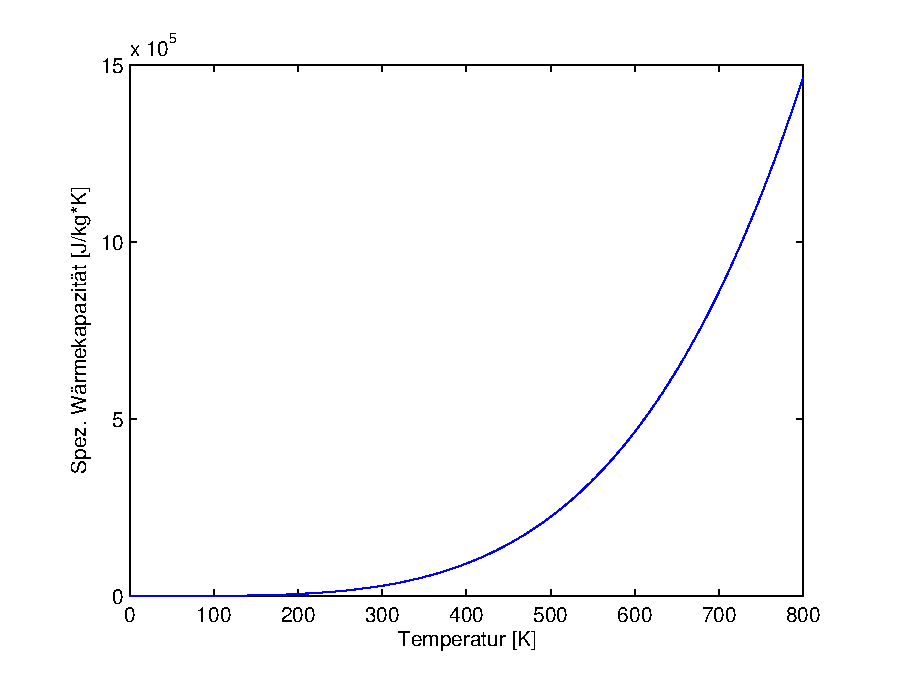
\includegraphics[width=0.8\textwidth]{cp_Plot.eps}
	\caption{Spez. Wärmekapazität temperaturabhängig} \label{fig:cpPlot}
	
\end{figure} 

Bei der Berechnung der isentropen Enthalpiedifferenz $\Delta H_{t_{is}}$ aus Gleichung \ref{eq:wgnenner} wurde $c_p$ nach Gleichung \ref{eq:cppolynom}
\begin{itemize}
	\item separat am In-/Outlet,
	\item aus dem arithmetischen Mittel der beiden Größen,
	\item in Abhängigkeit der isentropen Temperatur im Outlet
\end{itemize}
berechnet um den Einfluss der Berechnungsweise von $c_p$ auf die Berechnung des Wirkungsgrades zu analysieren.\\

Die verschiedenen Wirkungsgraddefinitionen in Abschnitt \ref{sec:wirkungsgrade} und Berechnungsweisen von $c_p$ wurden in CFX implementiert und miteinander verglichen. Das Ergebnis dieses Vergleichs wird im nächsten Abschnitt dargestellt.
%__________________________

\begin{comment}
\section{Wirkungsgrade bei der Aachen-Turbine}
\label{sec:wgaachen}
Bei der Aachen-Turbine ergaben sich je nach Berechnungsart folgende Werte für den Wirkungsgrad:
\begin{table}[H]
\centering
\caption{Wirkungsgrad bei der Aachen-Turbine}
\begin{tabular}{ c| c}
Berechnungsformel & $\eta$ \\
\hline
$\eta_{\Delta T_t}$ mit $c_p$ konstant& 86\% \\
$\eta_{\Delta T_t}$ mit $c_p(T)$& 86\% \\
$\eta_{\Delta h_t}$& 87\% \\
$\eta_{torque}$& 85\% \\
\end{tabular}
\label{tab:wgaachen}
\end{table}
Es ist zu sehen, dass .....
\todo
\end{comment}




%%% Local Variables: 
%%% mode: latex
%%% TeX-master: "main"
%%% End: 


 %Dominik Keijo eingefügt
	\chapter{Aachen-Turbine}
\label{cha:aachen}
Zur Analyse der verschiedenen Wirkungsgraddefinitionen wurde eine sogenannte Aachen-Turbine, das heißt eine Turbine mit einfachen Schaufeln ohne Krümmung in Radialrichtung, simuliert. In diesem Kapitel wird zunächst die Geometrie und die durchgeführte Gitterstudie vorgestellt. Danach werden die ermittelten Wirkungsgrade miteinander verglichen und Unterschiede vorgestellt.
\section{Geometrie}
\label{sec:aachengeo}
  \begin{figure}[htbp]
	\centering
	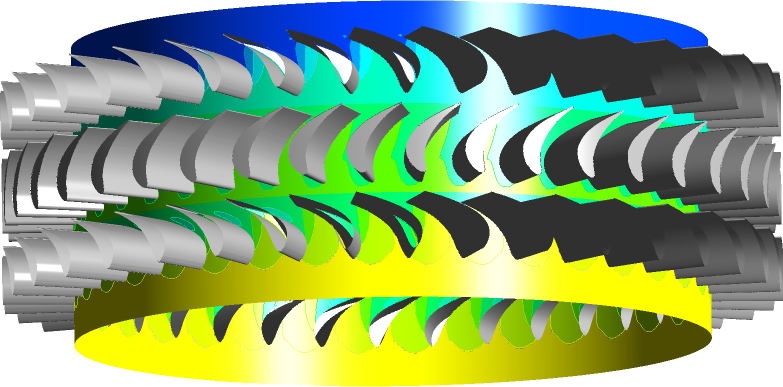
\includegraphics[width=0.8\textwidth]{AachenTurbine_trans.png}
	\caption{Aachen-Turbine} \label{fig:imgAachenTurbine}
\end{figure} 
Die verwendete Geometrie basiert auf der Aachen-Turbine, die auch in den Untersuchungen von \cite{ufi2001YaoDavis} 
verwendet wurde. Es werden dabei nur 1,5 Stufen berechnet, um den Rechenaufwand der Simulationen gering zu halten und den Vergleich der Wirkungsdefinitionen auch für diesen Aufbau möglich zu machen. Die Geometrie der Aachen-Turbine mit Gitter ist in der Abbildung \ref{fig:aachengebiet} zu sehen. 
\begin{figure}[htbp]
	\centering
	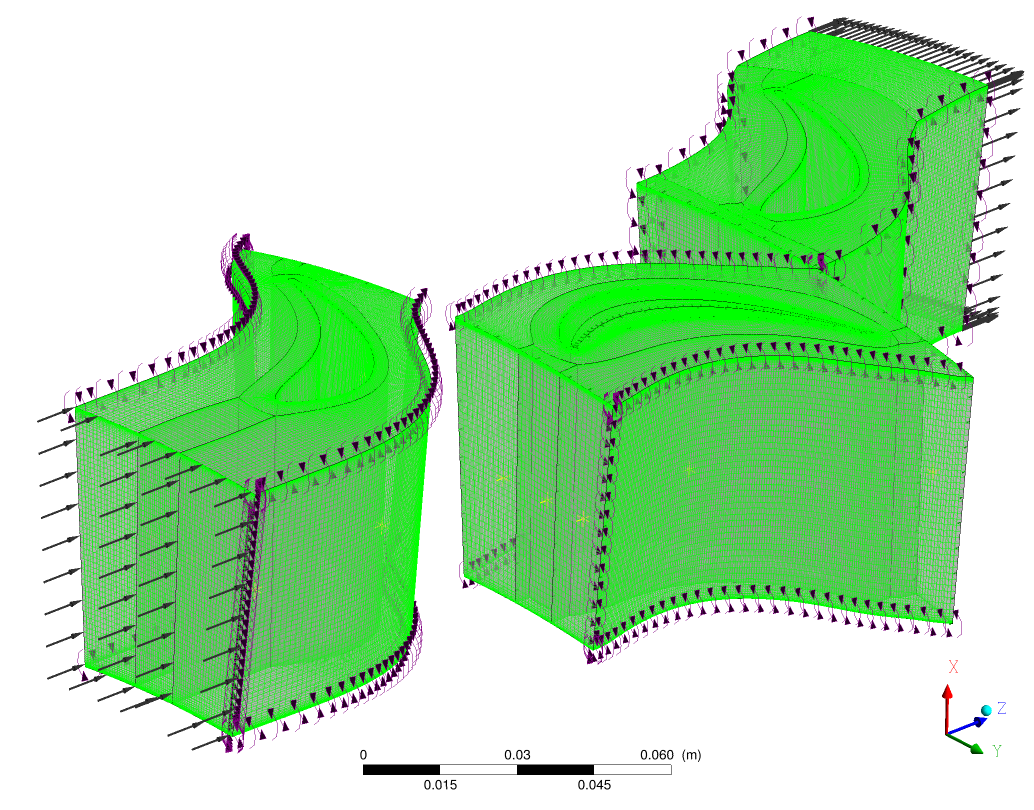
\includegraphics[width=0.7\textwidth]{aachenmitgitter.png}
	\caption{Eine dreidimensionale Ansicht der Aachen-Turbine mit Gitter.}
	\label{fig:aachengebiet}
\end{figure}
Die Aachen-Turbine besteht aus zwei Statoren und einem Rotor. Die erste Domäne als Stator mit Einstrom, die mittlere Domäne als Rotor und die letzte Domäne als zweiter Stator mit Ausstrom. Die Grenzen oben und unten stellen Shroud und Hub dar. Links und rechts herrschen periodische Randbedingungen. Die Statoren sind jeweils durch ein Interface mit dem Rotor verbunden. Die Anzahl an Schaufeln in Stator und Rotor sind der Tabelle \ref{tab:aachenabmessungen} zu entnehmen.\newline
\begin{table}[htbp]
\centering
\label{tab:aachenabmessungen}
\caption{Schaufelzahlen in Stator und Rotor}
\begin{tabular}{ c| c}
\# Schaufeln in Stator&\# Schaufeln in Rotor\\
\hline
36&41\\
\end{tabular}
\end{table}
Im folgenden Abschnitt wird der gewählte Betriebspunkt näher beschrieben.
%________________________________________________________
\section{Betriebspunkt}
\label{subsec:aachensetup}
Um den Betriebspunkt für die Simulationen dieser Arbeit festzulegen wird als Orientierung die Randbedingungen der Arbeit \glqq Unsteady Flow Investigations in an
Axial Turbine Using the Massively
Parallel Flow Solver TFLO\grqq \, \cite{ufi2001YaoDavis} zur Analyse der Aachen-Turbine übernommen. Diese sind der folgenden Tabelle \ref{tab:aachensetup} zu entnehmen.
\begin{table}[H]
\centering
\caption{Betriebspunkt} \label{tab:aachensetup}
\begin{tabular}{ c| c| c| c}
$T_{t_{Inlet}}$&$p_{t_{Inlet}}$&$Massenstrom$&$n_{Rotor}$\\
\hline
$305 \, K$&$\approx152.000 \, Pa$&$7 \, \frac{kg}{s}$&$3500 \, \frac{rev}{min}$\\
\end{tabular}
\end{table}
Der Totaldruck am Inlet wird als Druckprofil, siehe Abbildung \ref{fig:ptinlet}, entsprechend den Daten von \cite[p. 4]{ufi2001YaoDavis} angenommen
In den verschiedenen Aufgabenteilen werden die Eintrittsbedingungen jedoch auch verändert, um zum Beispiel den Einfluss inhomogener Eintrittsbedingungen oder höherer Temperaturen zu untersuchen.

\begin{figure}[H]
	\centering
	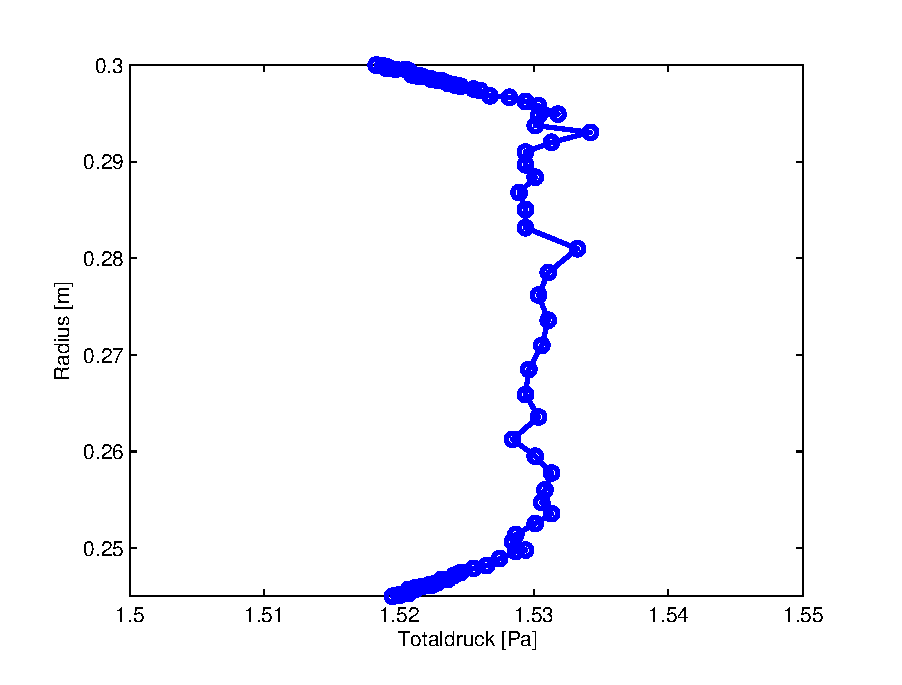
\includegraphics[width=0.7\textwidth]{PtInlet.eps}
	\caption{Totaldruck Profil Inlet} \label{fig:ptinlet}
\end{figure}


\section{Strukturiert}
Im Folgenden wird beschrieben, wie das strukturierte Netz der Aachen-Turbine erstellt wurde. Da das Netz Einfluss auf die numerische Konvergenz der Lösungsverfahren, auf die Qualität der Lösung, auf die Auflösung und damit auch auf den Diskretisierungsfehler hat, ist ein gutes Netz von großer Bedeutung. Deshalb wurde eine Netzstudie - basierend auf einem Referenzgitter – durchgeführt und anschließend das bestmögliche Netz in Bezug auf Qualität vs. geringe Anzahl an Gitterzellen ausgewählt. 

\subsection{Erstellung des Gitters}

Zunächst wurde das Referenzgitter erstellt. Dazu wurde die Geometrie der Aachen-Turbine mittels des strukturierten Multi-Block Netzgenerators AutoGrid5 vernetzt. Dieser ist speziell für die Vernetzung von Turbomaschinen ausgelegt. 
Da die uns zur Verfügung stehende Vorlage der Aachen-Turbine die 1,5 Stufen zusammenhängend beinhaltete, erzeugten wir zu Beginn jeweils einzelne Gitter für Stator1, Rotor und Stator2 um diese später in CFX verwenden zu können. Hierbei wurde jeweils erst ein Vernetzungsdurchlauf basierend auf den voreingestellten Standartwerten durchgeführt und anschließend manuell optimiert. Für eine ausreichend gute Netzqualität dürfen bestimmte Netzkriterien nicht verletzt werden. Andernfalls kann es sein, dass die Lösung nicht, oder nur schlecht konvergiert. In unserem Fall haben wir darauf geachtet, dass wir keine negativen Kontrollvolumina haben, dass die kleinsten Winkel in einer Zelle größer 20° sind, dass das Expansionratio - welches das Volumenverhältnis zweier Zellen beschreibt – kleiner als 2.3 ist und dass das Aspectratio – welches das Verhältnis von längster zu kürzester Seite einer Zelle angibt – unter 1500 ist. Variiert wurden hauptsächlich die Anzahl und die Verteilung der Zellen in der B2B Ansicht. Diese stellt einen Querschnitt durch die Schaufel dar. In radialer Richtung wurde die Zellenverteilung im „flowpath“ angepasst. 

\subsection{Spaltverfeinerung}

Zur Bestimmung der Gitterauflösung im Spalt des Rotors wurde zudem die Anzahl der Zellen im Spalt variiert. Es stellte sich heraus, dass im Vergleich zum ursprünglichen Gitter mehr Zellen hinzugefügt werden mussten, da die Auflösung nicht fein genug war und man Änderungen im Vergleich zur gröberen Auflösung sah.  In den Abbildungen \ref{effSpalt1} und \ref{effSpalt15} ist die Gitterstudie für den Spalt mit 1 und 1,5 Stufen dargestellt. \todo welches Gitter ausgewählt, 3.?


\begin{figure}[htbp]
	\centering
	\label{effSpalt1}
	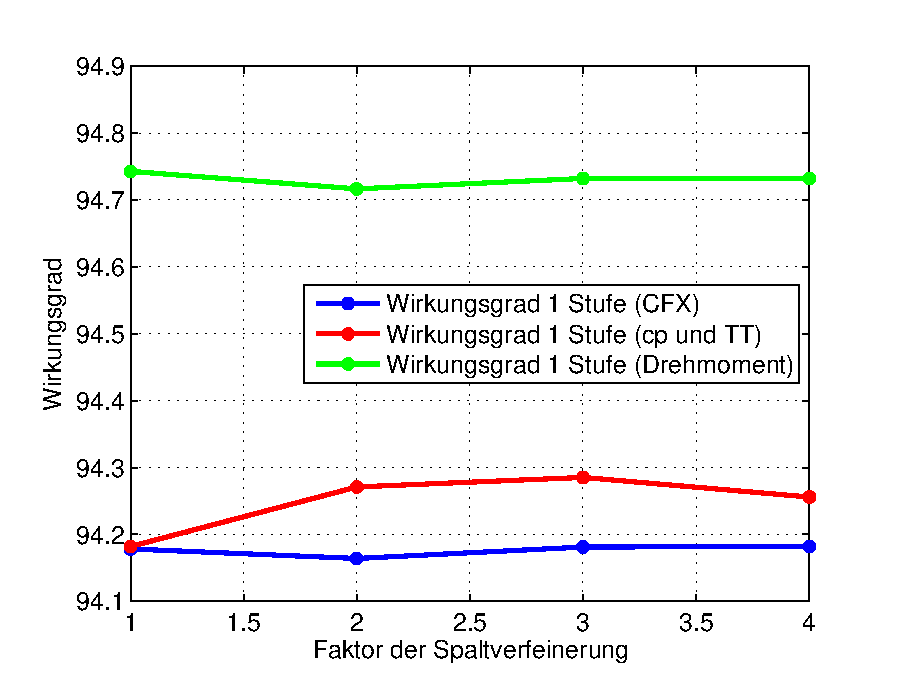
\includegraphics[width=0.7\textwidth]{efficiencySpalt1Stufe.eps}
	\caption{Gitterstudie des Spalts für eine Stufe}
\end{figure}

\begin{figure}[htbp]
	\centering
	\label{effSpalt15}
	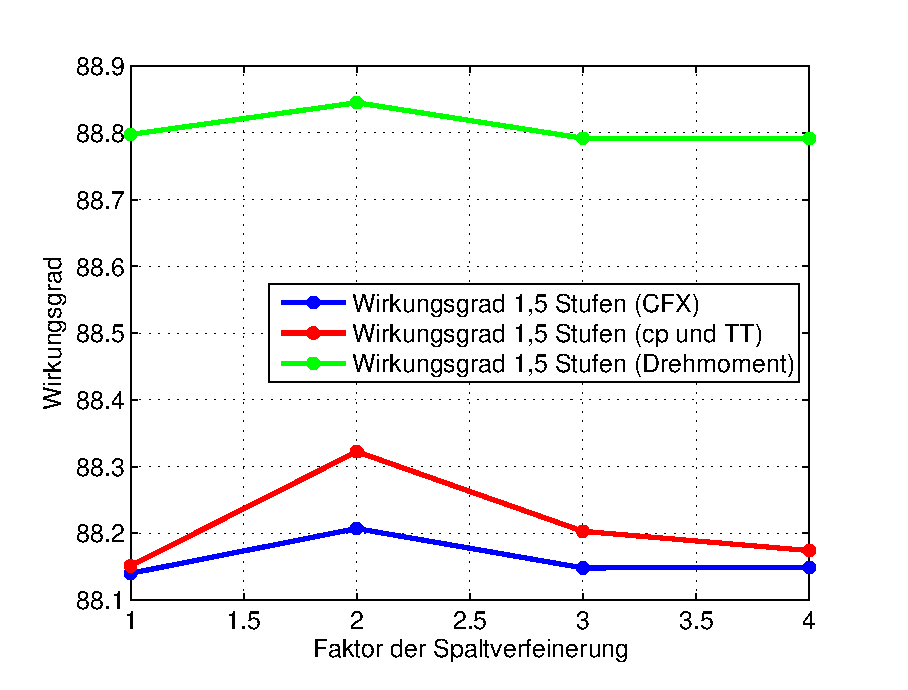
\includegraphics[width=0.7\textwidth]{efficiencySpalt15Stufen.eps}
	\caption{Gitterstudie des Spalts für 1,5 Stufen}
\end{figure}

\subsection{Einstellen der Grenzschichtdicke}
Außerdem musste noch die Grenzschichtdicke, bzw. das y-plus eingestellt werden. Die Strömung wurde bis in die viskose Unterschicht aufgelöst, sodass die Auflösung in Wandnähe im Bereich der kleinsten Wirbel liegt. Das Verhältnis der Grenzschichtdicke zu den kleinsten Wirbeln sollte kleiner als 1 sein. \todo Formel einfügen. Um das korrekte y-plus zu bestimmen, haben wir die Werte in AutoGrid für den Wandabstand sowohl auf dem Schaufelrand im B2B-Layer, als auch an Hub und Shroud variiert.  Anschließend haben wir eine Simulation in CFX durchgeführt und dann die Verteilung des y-plus-Wertes über die Schaufel hinweg visualisiert und ausgewertet. Schließlich kamen wir zu dem Ergebnis, dass die optimale Grenzschichtdicke für den Rotor bei $2e-6$ im Flowpath an Hub und Shroud und bei $1.5e-6$ am Blade liegt. Die kompletten Werte sind in Tabelle \ref{cellWidths} zu sehen. Über die komplette Schaufel betrachtet liegen die y-plus-Werte in einem Bereich von $0.3 \leq y^+ \leq 3$ nahezu überall. Da man nur wenige Stellschrauben zur Beeinflussung dieses Wertes in AutoGrid hat, ist dieser Wertebereich zufriedenstellend, zumal die Mehrheit der Werte im Bereich von $0.7 \leq y^+ \leq 1.2$  liegt, wie in Abb. \ref{imgYplusWerte} zu sehen ist. 

\begin{table}[t]
\centering
\begin{tabular}[t]{cccc}
\toprule
 Cell width  & Stator1 & Rotor & Stator2  \\
\midrule
Cell width at Hub & 2.7e-6 & 2e-6 & 1.4e-6\\
Cell width at Shroud & 2.7e-6 & 2e-6 & 1.4e-6 \\
Cell width at Wall (Blade) & 1.56e-6 & 1.5e-6 & 1.7e-6 \\
\bottomrule
\end{tabular}
\caption{Zellgrößen an der Wand für Rotor und die Statoren}
\label{cellWidths}
\end{table}

\begin{figure}[htbp]
	\centering
	\label{imgYplusWerte}
	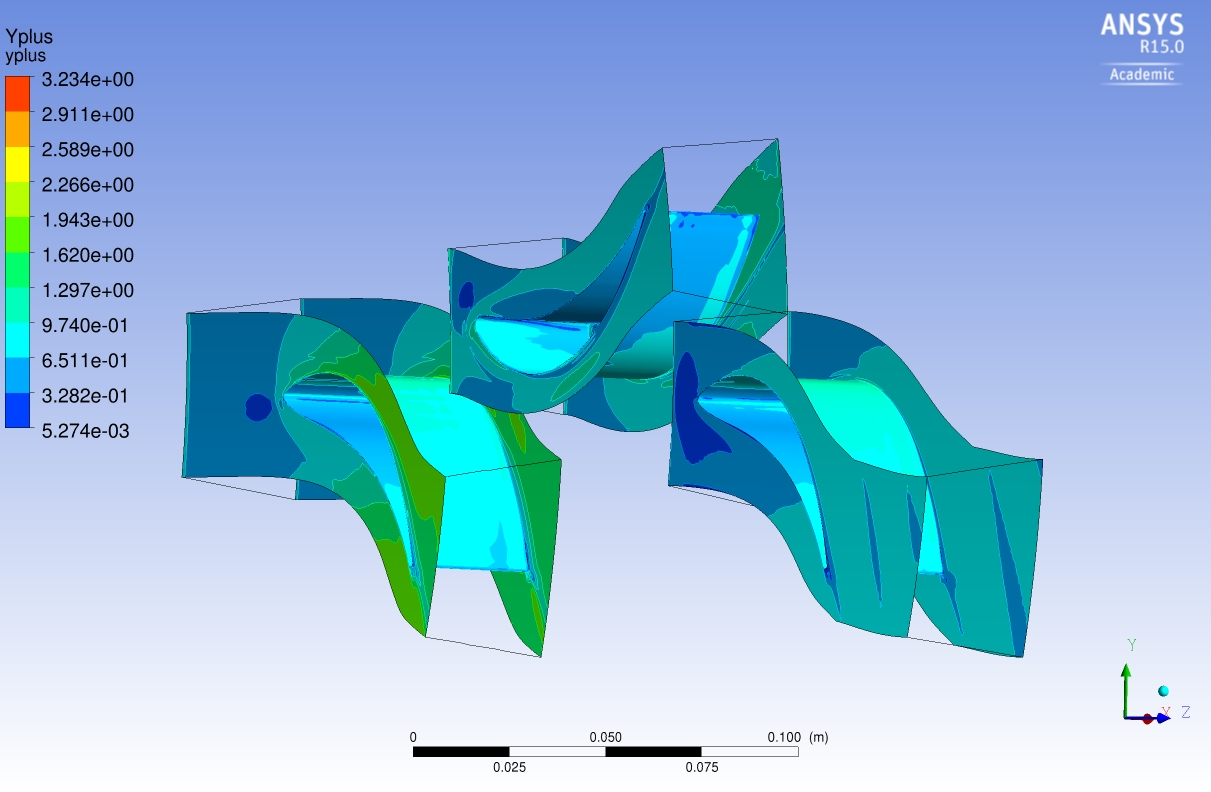
\includegraphics[width=0.7\textwidth]{yPlus.jpg}
	\caption{$y^+$-Verteilung über die komplette Stufe}
\end{figure}

\subsection{Durchführung der Netzstudie}

Nachdem nun ein Referenzgitter mit guter Gitterqualität und korrekter Grenzschichtdicke vorhanden war, konnte die eigentliche Netzstudie durchgeführt werden um die minimale Auflösung zu bestimmen, die das Netz haben muss, damit die Lösung netzunabhängig ist. Hierzu wurde das Referenzgitter sowohl gröber aufgelöst, als auch verfeinert und dann der Einfluss auf verschiedene Größen, die z.B. die Wirkungsgrade verglichen. Sobald sich dieser im Vergleich zum nächst feineren, bzw. nächst gröberen Gitter kaum noch ändert, ist die Lösung von der Gitterdiskretisierung unabhängig. 
Insgesamt wurden 7 verschiedene Verfeinerungsstufen erstellt und simuliert. Das Referenzgitter hat jeweils knapp 1 Million Zellen für Rotor und die Statoren. Zunächst wurde versucht, die Zellenanzahl zu verdoppeln. Dazu wurde die Auflösung in allen drei Raumrichtungen mit $\sqrt[3]{2}$ multipliziert um insgesamt einen Faktor von 2 zu erlagen. Dies wurde dann nochmal wiederholt, um einen Faktor 4 gegenüber dem Referenznetz zu erreichen. Außerdem wurde das Referenznetz auf die halbe Zellenanzahl halbiert. Mit den Ergebnissen, dieser 4 Simulationen wurde bereits versucht, eine Aussage über die Netzunabhängigkeit zu treffen. Allerdings war hier noch nicht ganz ersichtlich, welches Netz hier genommen werden konnte, da die Unterschiede noch zu groß waren. Allerdings sah das 2x Gitter schon sehr gut aus. Daraufhin führten wir noch drei weitere Simulationen durch, jeweils mit den Auflösungen 1.3x, 1.5x und 3x in Bezug zum Referenzgitter. Nun war zu erkennen, dass das Netz mit der doppelten Auflösung praktisch unabhängig war, sodass wir dieses als unser Gitter für die nachfolgenden Rechnungen definieren konnten. 
\todo Kenngrößen des Gitters hinschreiben + Plots einfügen


\subsection{Fillets}

In realen Turbinen befinden sich an der Schaufel am Übergang zum Randbereich sogenannte Fillets, also Verrundungen, um bessere Strömungseigenschaften zu erhalten, Ablöseblasen zu vermeiden und bessere Festigkeitseigenschaften zu erhalten. Daher wurde auch eine Simulation der Aachen-Turbine mit Fillets durchgeführt, das Netz ist in Abb. \ref{imgFillet1} zu sehen. Jedoch ergab sich das Problem, dass nur sehr kleine Fillets erstellt werden konnten, da die Statoren eine „Delle“ an der Vorderkante aufweisen, wie in Abb. \ref{imgFilletDelle} zu sehen ist und daher ab einem bestimmten Radius negative Kontrollvolumen durch die Fillets entstehen. Jedoch wurde eine Simulation mit einem Fillet des Radius 0.00055 durchgeführt. Es hat sich herausgestellt, dass die Gitterqualität wesentlich schlechter wurde, da mehr schrägwinklige Zellen im Filletbereich notwendig wurden. Allerdings wurde auch der y-plus-Wertebereich etwas besser, da sehr kleine und sehr große Werte verschwanden.     

  \begin{figure}[htbp]
	\centering
	\label{imgFillet1}
	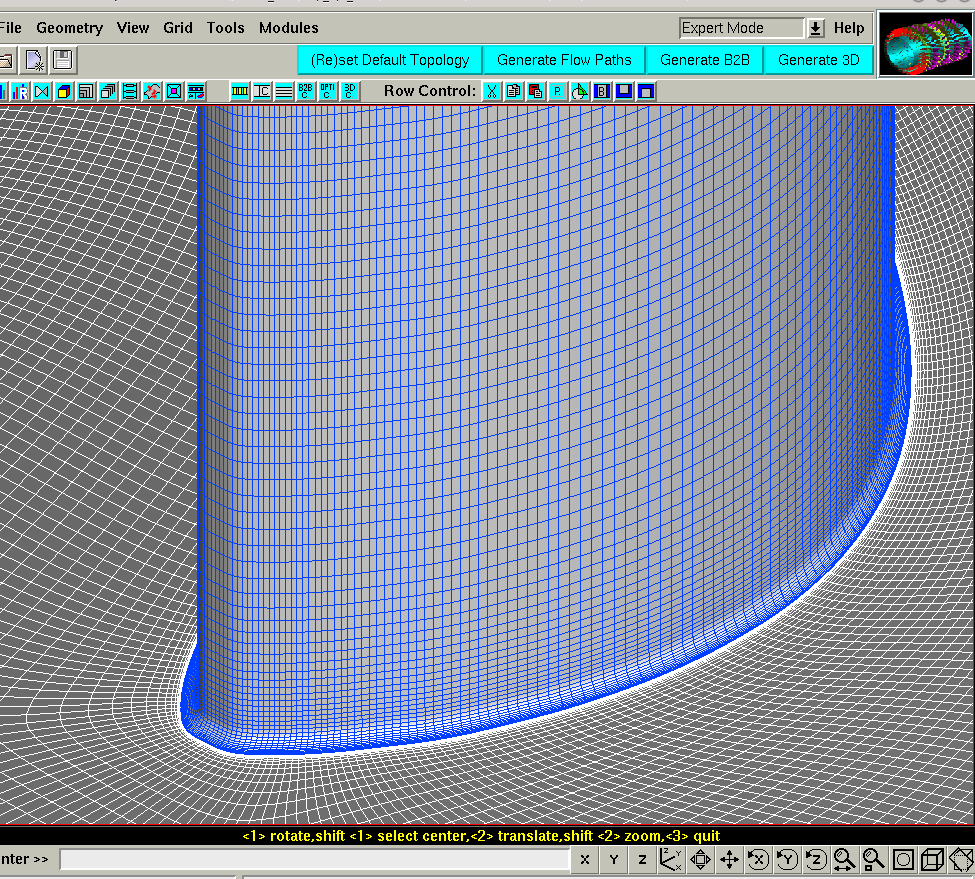
\includegraphics[width=0.7\textwidth]{fillet0_00055.png}
	\caption{Netz mit Fillet der Größe 0.00055}
\end{figure} 

  \begin{figure}[htbp]
	\centering
	\label{imgFilletDelle}
	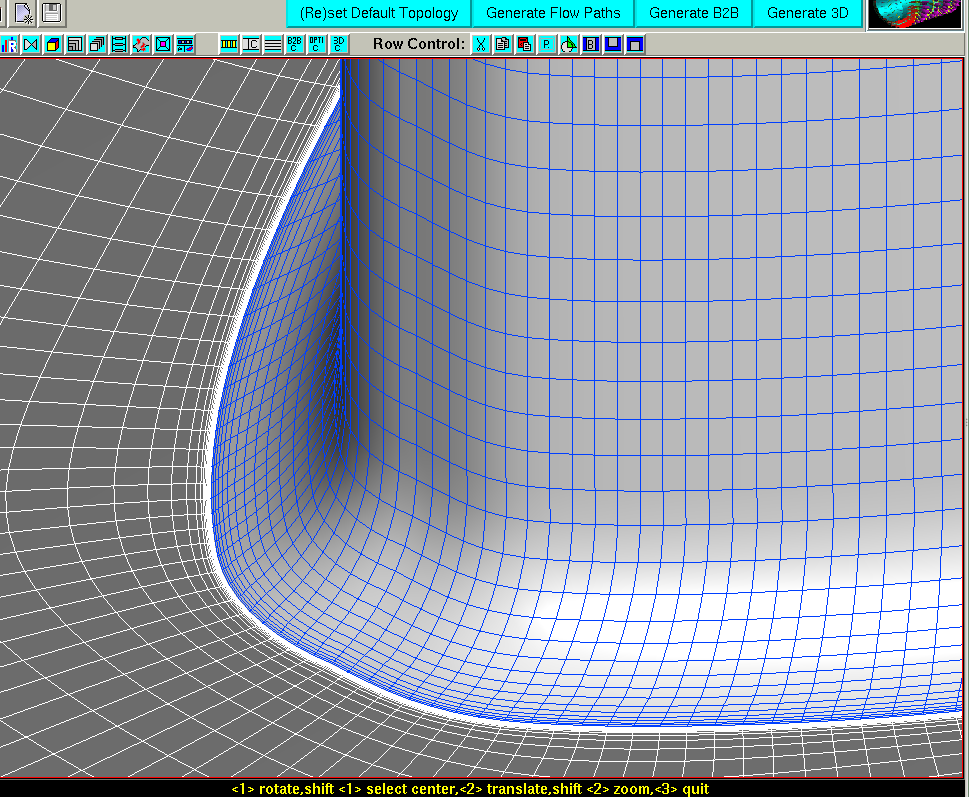
\includegraphics[width=0.7\textwidth]{filletDelle.png}
	\caption{Delle in der Statorgeometrie}
\end{figure} 
\section{Unstrukturiertes Gitter}
Um generelle Unterschiede zwischen einem strukturierten und unstrukturierten Gitter festzustellen, wurden zusätzlich Berechnungen mit einem unstrukturierten Gitter durchgeführt.

\subsection{Aufgetretene Probleme}
Für den zweiten Stator liegt kein CAD-File, lediglich eine Netzdatei vor. Somit war es nicht möglich ein unstrukturiertes Gitter für diesen zu erstellen. Für die Berechnungen wurde daher das Gitter der Aachen-Turbine teilweise unstrukturiert und strukturiert betrachtet.\\
Die Erstellung der unstrukturierten Gitter war aufgrund von Lizenzproblemen nicht immer möglich, was die Anzahl der durchgeführten Simulationen eingrenzt.
\subsection{Erstellung des Gitters}
Das unstrukturierte Gitter wurde mit Centaur erstellt. Zunächst wurde ein Referenzgitter mit den Standardwerten gebildet. Für das Einstellen von $y^+$ wurde zunächst der gleiche Wandabstand wie im Falle des strukturierten Gitters verwendet. Nach einem ersten Test wurde dieser im Rotor verringert. Die Verteilung von $y^+$ des ersten Stators und Rotors ist in Abbildung \ref{yplusunstrukturiert} dargestellt.
\begin{figure}[htbp]
	\centering
	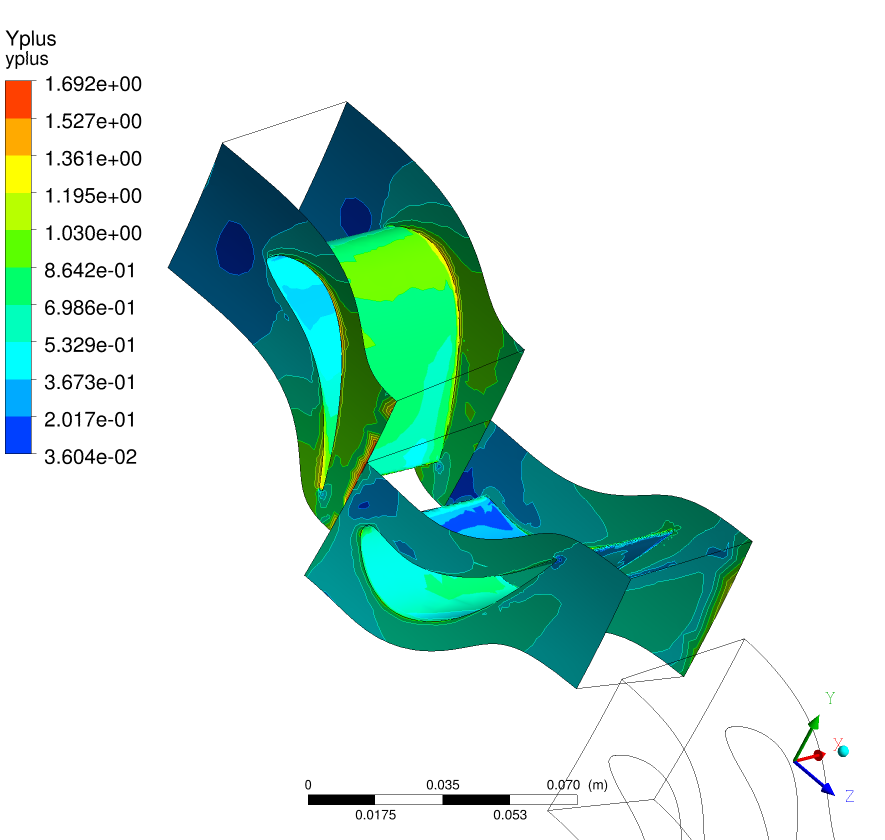
\includegraphics[width=0.7\textwidth]{yplusunstrukturiert.png}
	\caption{$y^+$ des unstrukturierten Gitters} \label{yplusunstrukturiert}
\end{figure}
\subsubsection{Verwendung von Sources}
Um das Gitter lokal an bestimmten Stellen zu verfeinern wurden  sogenannte Sources mit Hilfe Centaur eingeführt.
Eine davon regelt die unterschiedlichen Wandabstände von Schaufel, Nabe und Gehäuse.\\
Eine weitere Source verfeinert die Zellen im Nachlauf der Schaufel relativ zu den umliegenden Zellen um den Faktor $c = 0.8$.

\subsection{Gitterstudie}
Zuerst wurde der Spalt des Rotors wie beim strukturierten Gitter verfeinert. Anschließend wurde eine Gitterstudie mit verschiedenen Verfeinerungsstufen, siehe Tabelle \ref{tab:verfeinerungenunstrukturiert}, durchgeführt. In den Abbildungen \ref{fig:gitterunstrukturiert1stufe} und \ref{fig:gitterunstrukturiert15stufen} ist der Wirkungsgrad in \% über die Verfeinerungsstufen aufgetragen. Es ist zu erkennen, dass die Wirkungsgrade weiterhin in Abhängigkeit der Kontrollvolumenzahl steigen. Damit eine netzunabhängige Lösung ermittelt werden kann, müssten weitere Verfeinerungsstufen zwischen 2 und 3 und größer 3 gerechnet werden, bis kein Ansteigen oder Absinken mehr zu erkennen ist. Dies war aufgrund von Lizenzproblemen nicht möglich.\\
Für die Berechnungen mit einem temperaturabhängigen $c_p$ und für die Vergleiche mit dem strukturierten Gitter wurde das feinste Netz verwendet.
\begin{table}[h]
		\centering
		\caption{Verfeinerungsstufen des unstrukturierten Gitters}
	\begin{tabular}{ c| c | c| c| c}
Verfeinerungsstufe	&	Stator 1	&		&	Rotor	&		\\
&	Anzahl Knoten	&	Anzahl Elemente	&	Anzahl Knoten	&	Anzahl Elemente	\\
\hline									
0,5	&	61435	&	174098	&	281782	&	724470	\\
1	&	147399	&	473211	&	638948	&	1741931	\\
2	&	244772	&	880367	&	1007020	&	2835297	\\
\textbf{3}	&	\textbf{1196277}	&	\textbf{6457352}	&	\textbf{1880370}	&	\textbf{6844537}	\\

	\end{tabular}
		\label{tab:verfeinerungenunstrukturiert}
\end{table}
\begin{figure}[htbp]
	\centering
	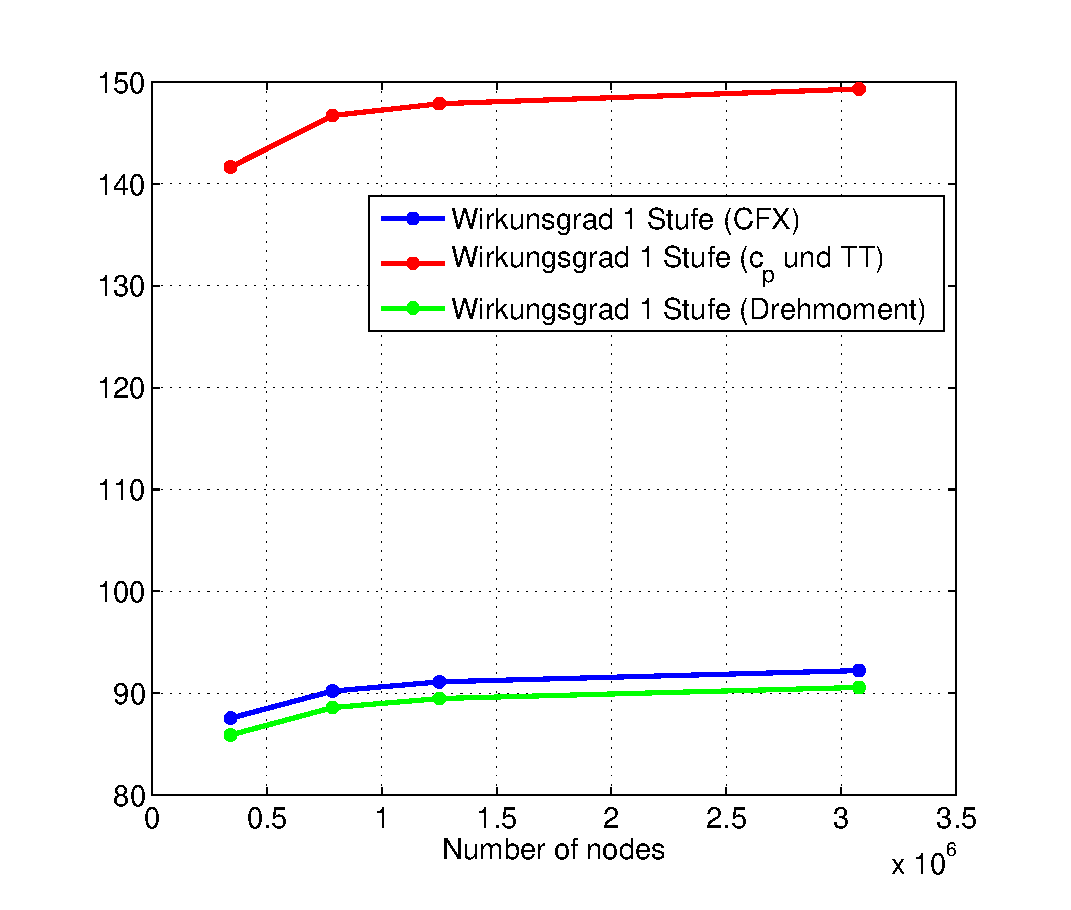
\includegraphics[width=0.7\textwidth]{gitterstudieunstrukturiert1stufe.eps}
	\caption{Gitterstudie des unstrukturierten Gitters für eine Stufe} \label{fig:gitterunstrukturiert1stufe}
\end{figure}

\begin{figure}[htbp]
	\centering
	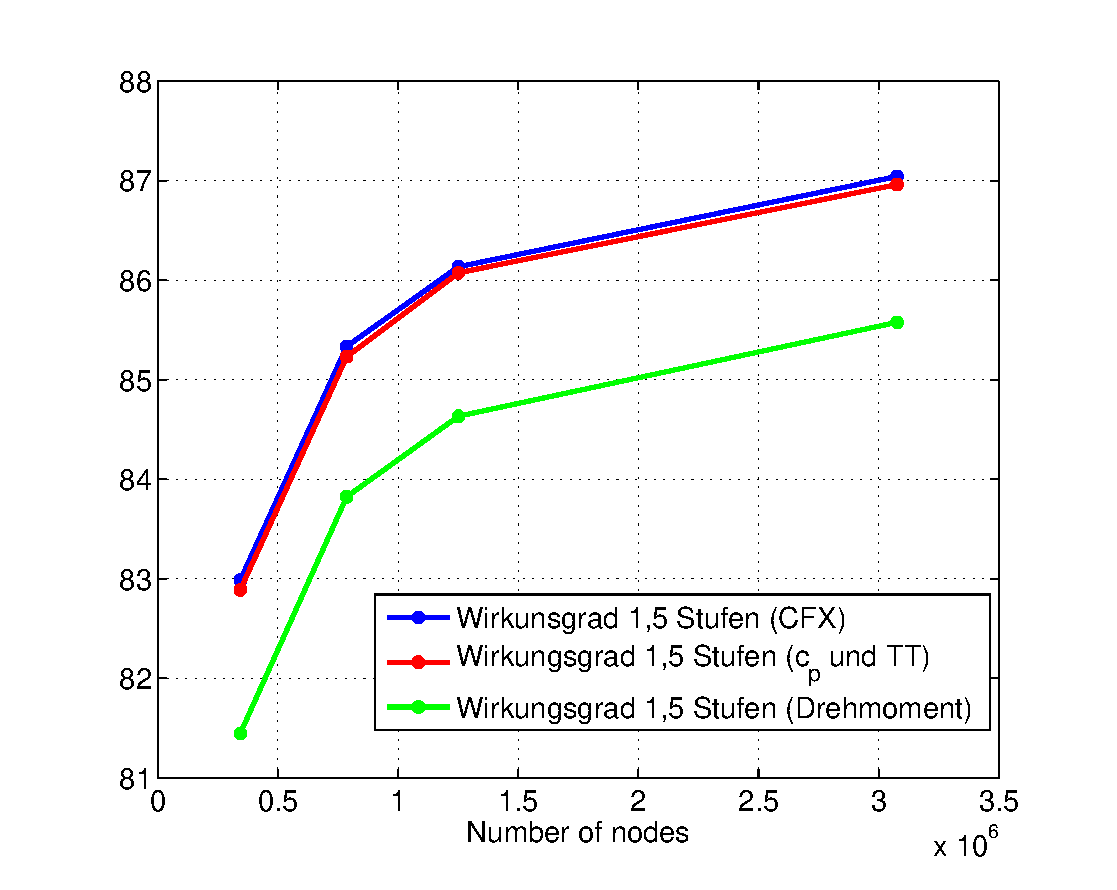
\includegraphics[width=0.7\textwidth]{gitterstudieunstrukturiert15stufen.eps}
	\caption{Gitterstudie des unstrukturierten Gitters für 1,5 Stufen}
	\label{fig:gitterunstrukturiert15stufen}
\end{figure}
\section{Vergleich der Wirkunsgrade}
Bei der Aachen-Turbine ergaben sich je nach Berechnungsart folgende Werte für den Wirkungsgrad:
\begin{table}[H]
	\centering
	\caption{Wirkungsgrad bei der Aachen-Turbine}
	\begin{tabular}{ c| c | c}
Berechnungsformel	&	$\eta_{strukturiert}$	&	$\eta_{unstrukturiert}$	\\
\hline
1 Stufe	&		&		\\
\hline
$\eta_{CFX}$	&	$92,33\%$	&	$92,23\%$	\\
$\eta_{c_p, T_t}$	&	$92,44\%$	&	$92,23\%$	\\
$\eta_{torque}$	&	$92,87\%$	&	$90,58\%$	\\
\hline
1,5 Stufen 	&		&		\\
\hline
$\eta_{CFX}$	&	$86,42\%$	&	$87,05\%$	\\
$\eta_{c_p, T_t}$	&	$86,48\%$	&	$87\%$	\\
$\eta_{torque}$	&	$87.05\%$	&	$85,58\%$	\\

	\end{tabular}
	\label{tab:wgaachen}
\end{table}
In Tabelle \ref{tab:wgaachen} werden die Wirkungsgrade des strukturierten und des unstrukturierten Gitters dargestellt. Diese weichen höchstens um $1,7\%$ voneinander ab. Es ist zu erkennen, dass die Wirkungsgrade im strukturierten Fall bei einer Stufe bis zu zwei Prozentpunkten größer sind. Bei der Betrachtung von 1,5 Stufen ist dagegen zu erkennen, dass die Wirkungsgrade im strukturierten Fall um $0,6$ Prozentpunkte kleiner sind.\\
Dies kann an dem Übergang vom Rotor in den zweiten Stator liegen. Dort findet ein Wechsel des Gitters von unstrukturiert nach strukturiert statt.\\
Allerdings ist die durchgeführte Gitterstudie im unstrukturierten Fall nicht zufriedenstellend durchgeführt, was in den Abbildungen \ref{fig:gitterunstrukturiert1stufe} und \ref{fig:gitterunstrukturiert15stufen} zu erkennen ist. Daher fällt ein Vergleich der beiden Gittertypen schwer und ist nicht aussagekräftig. \\ 

Aus den physikalischen Grundlagen zur Berechnung des Wirkungsgrades ist nach dem Satz der Massenerhaltung der Massenstrom über die gesamte Turbine konstant.
Aufgrund numerischer Faktoren, sowie konstruktionsbedingt kann es jedoch zu Veränderungen im Massenstrom kommen. 
Insbesondere kommt es an den Verbindungsstellen der einzelnen Domänen zu Abweichungen. Hierzu wird in Kapitel \ref{cha:kanal} näher eingegangen.
Auffällig ist jedoch, dass es hierbei gravierende Unterschiede im Hinblick auf die Gitterstrukturierung gibt. In Abbildung \ref{fig:massFlowUnstrukt} ist der Verlauf des Massenstroms durch die Turbine dargestellt. Die Position in der Turbine ist auf der Abszisse dargestellt, die Interfaces befinden sich bei 1 und 2. Auf der Ordinate ist der jeweilige Massenstrom aufgetragen. Für die unstrukturierte Vernetzung treten Massenstromunterschiede von $0,1664 \frac{kg}{s}$ auf. Im Vergleich dazu liegt die Massenstromabweichung für das strukturierte Gitter, siehe Abbildung \ref{fig:massFlowStrukt}, lediglich bei $0.00028\frac{kg}{s}$.

 \begin{figure}[htbp]
	\centering
	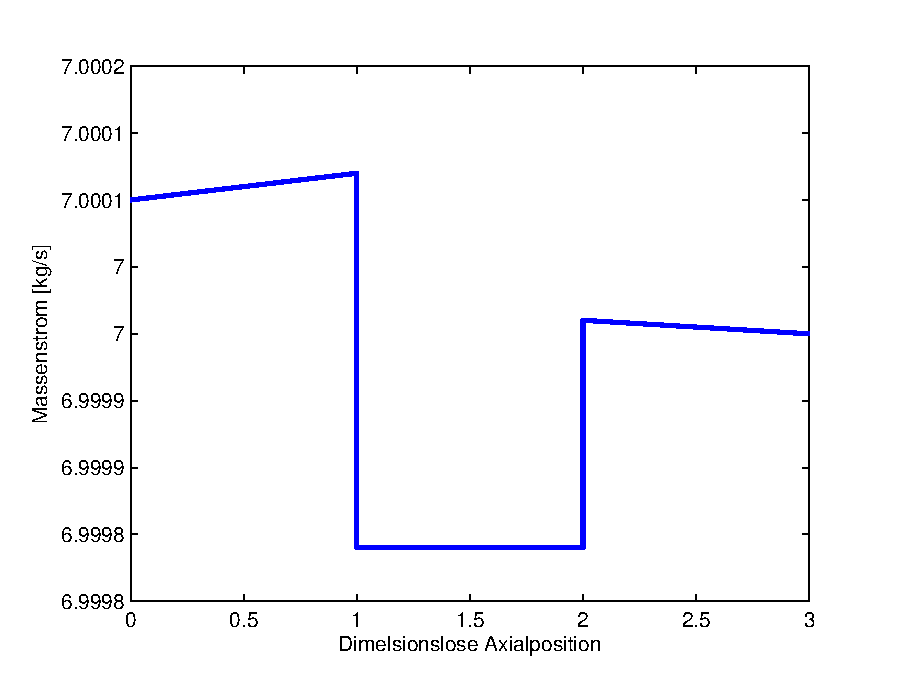
\includegraphics[width=0.8\textwidth]{massFlow_strukt_1.eps}
	\caption{Massenstrom in der Turbine, strukturiertes Gitter} \label{fig:massFlowStrukt}
\end{figure} 
 \begin{figure}[htbp]
	\centering
	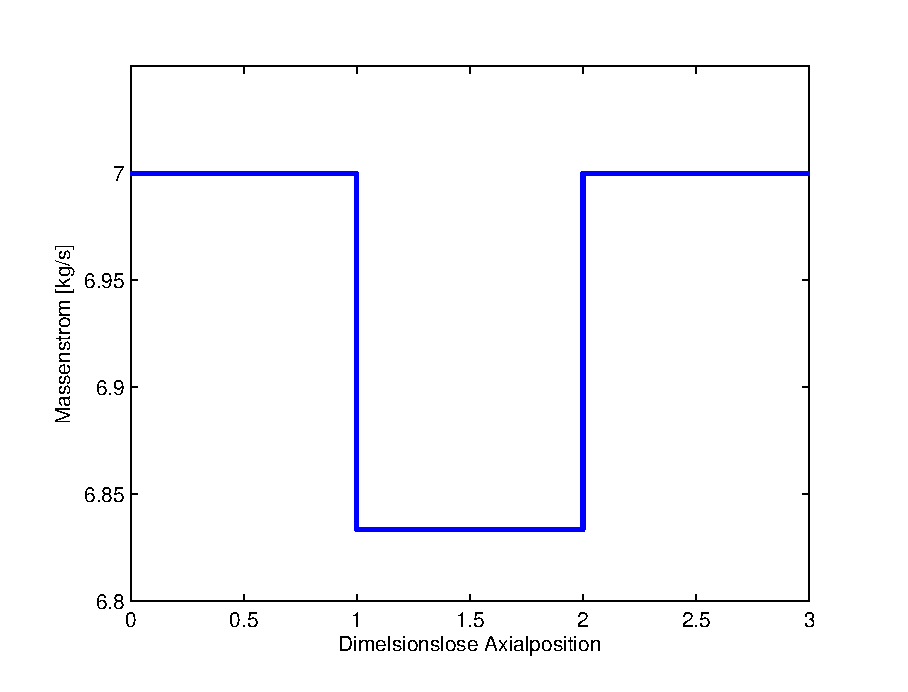
\includegraphics[width=0.8\textwidth]{massFlow_unstrukt_1.eps}
	\caption{Massenstrom in der Turbine, unstrukturiertes Gitter} \label{fig:massFlowUnstrukt}
\end{figure} 
\subsection{Wirkungsgrade mit temperaturabhängigem $c_p$}
\begin{table}[H]
	Für die Untersuchung der Wirkungsgrade unter Berücksichtigung der spezifischen Wärmekapazität in Abhängigkeit der Temperatur wurden die Definitionen aus Kapitel \ref{subsec:spezWK} verwendet. 
	Als Resultate ergeben sich die Wirkungsgrade in Tabelle \ref{tab:strukturiertmycp} und \ref{tab:unstrukturiertmycp}. Hierbei ist durchaus eine Veränderung zu beobachten, welche jedoch nur teilweise auf die nun verwendete spezifische Wärmekapazität zurückzuführen ist. Ein größerer Faktor für die Veränderung der Wirkungsgrade ist die zu beobachtenden Änderungen des Massenstroms und die unterschiedliche Definition der verwendeten Wirkungsgrade. Für die Isentrope Leistung wird immer der Massenstrom gemessen am Einlauf der Turbine verwendet, während für den Wirkungsgrad $\eta_{c_p, T_t}$ zur Berechnung der erzeugten Leistung die lokalen Massenströme an Einlauf und Auslauf verwendet werden. selbst kleine Schwankungen des Massenstroms führen hierbei zu gravierenden Änderungen im Wirkungsgrad.
	
	\centering
	\caption{Vergleich der Wirkungsgraddefinitionen auf einem strukturierten Gitter mit $c_p = f(T)$}
	\begin{tabular}{ l| c | c c c c}
		&	$c_p = const.$	&	$c_p(T)$	&		&		&		\\
		\hline
		&		&	$c_p^*$	&	$\overline{c_p^*}$	&	$\overline{c_p}$	&	$c_p$	\\
		\hline
		$\eta_{CFX}$	&	81,24 \%	&	53,89\%	&	79,19 \%	&	79,19 \%	&	60,25\%	\\
		$\eta_{c_p, T_t}$	&	81,25\%	&	74,6 \%	&	78,3 \%	&	78,07\%	&	83,41 \%	\\
	$\eta_{torque}$	&	82,52\%	&	54,35 \%	&	80,11 \%	&	79,87 \%	&	60,77\%	\\
		
	\end{tabular}
	\label{tab:strukturiertmycp}
\end{table}

\begin{table}[H]
	\centering
	\caption{Vergleich der Wirkungsgraddefinitionen auf einem unstrukturierten Gitter mit $c_p = f(T)$}
	\begin{tabular}{ l| c | c c c c}
		&	$c_p = const.$	&	$c_p(T)$	&		&		&		\\
		\hline
		&		&$c_p^*$	&	$\overline{c_p^*}$	&	$\overline{c_p}$	&	$c_p$	\\
		\hline
		$\eta_{CFX}$	&	80,21 \%	&	71,93 \%	&	77,96 \%	&	78,34 \%	&	60,01 \%	\\
		$\eta_{c_p, T_t}$	&	80,1 \%	&	\textcolor{red}{100,36} \%	&	78,23 \%	&	78,61\%	&	83,72 \%	\\
		$\eta_{torque}$	&	79,5 \%	&	70,23 \%	&	77,1 \%	&	77,48 \%	&	59,36 \%	\\
		
	\end{tabular}
	\label{tab:unstrukturiertmycp}
\end{table}
%%% Local Variables: 
%%% mode: latex
%%% TeX-master: "main"
%%% End: 


 %Dominik Keijo eingefügt
	\chapter{Einfluss inhomogener Randbedingungen und des Stator-Rotor Interface auf die Wirkungsgradbestimmung}
\label{cha:kanal}
Bei der Berechnung des Wirkungsgrades führen geringe Abweichungen der Totaltemperatur zu großen Änderungen des Wirkungsgrades. An dem Stator-Rotor Interface kommt es bei Wahl einer sogenannten Mixing-Plane zur stationären Berechnung zu einem Ansteigen der Totaltemperatur. In diesem Kapitel wird zunächst die Funktionsweise der Mixing Plane erläutert und die Ergebnisse der Analyse des Einflusses der Mixing Plane bei unterschiedlichen Einstrombedingungen vorgestellt.
%______________________________________________________
\section{Mixing Plane / Stage}
In dem verwendeten Setup der Aachenturbine werden die 1 1/2 Stufen in drei Domänen dargestellt. Hierbei kommt es zu einer Herausforderung; die Domänen müssen miteinander verbunden werden. Um dies zu bewerkstelligen, werden jeweils an den Verbindungsstellen von Stator zu Rotor und Rotor zu Stator sogenannte \textit{Interfaces} definiert.
Im Falle einer solchen Anordnung ist in CFX die \textit{General Connection} zu wählen, da sich rotierende an stationäre Domänen anschließen.\\
Eine Möglichkeit ein solches Interface mittels General Connection zu definieren ist das Frozen Rotor Interface. Hierbei bleibt die relative Orientierung der Komponenten über die gesamte Berechnung erhalten. 
Dieses Modell hat seine Vorteile bei großen Schwankungen der Strömungsgrößen in Umfangsrichtung.\\
Eine weitere Untergruppe der \textit{General Connection} in CFX ist das Stage- oder Mixing Plane-Interface, welches für die Erstellung des in dieser Arbeit verwendeten Setups eingesetzt wird. Hierbei werden die Strömungsgrößen an der Verbindungsstelle über den Umfang gemittelt.
Durch die Mittelung der Strömungsgrößen am Interface treten Vermischungsverluste auf. Laut ANSYS sind die hierbei entstehenden Verluste äquivalent zu den physikalischen Vermischungseffekten der zwischen Stator und Rotor und eines somit entstehenden Geschwindigkeitsprofils in entgegen der Strömungsrichtung.\\
%Quelle: \url{
TODO ${https://www.sharcnet.ca/Software/Ansys/17.0/en-us/help/cfx_mod/CACDIGEH.html} $- 12.06.2017 TODO
%_____________________________________________________________________
\section{Rohrauschnitt}
\label{sec:kanalgeo}
Anstelle der Aachen-Turbine wurde für die Analyse des Stator-Rotor Interface ein Rohrausschnitt, geteilt in Stator und Rotor, berechnet, um den Einfluss des Interfaces auf die Strömungsgrößen in Hinblick auf die Wirkungsgradberechnung zu testen. Dabei wurden die Eintrittsbedingungen verändert und das Verhalten der Mixing-Plane unter unterschiedlichen Anströmbedingungen untersucht. In den folgendem Abschnitt wird zunächst das Rechengebiet näher beschrieben.
%________________________________________________________
\subsection{Problemgebiet}
\label{subsec:kanalproblemgebiet}
Die Geometrie des Rohrausschnitts mit Gitter ist in der Abbildung \ref{fig:kanalgebiet} zu sehen.
\begin{figure}[H]
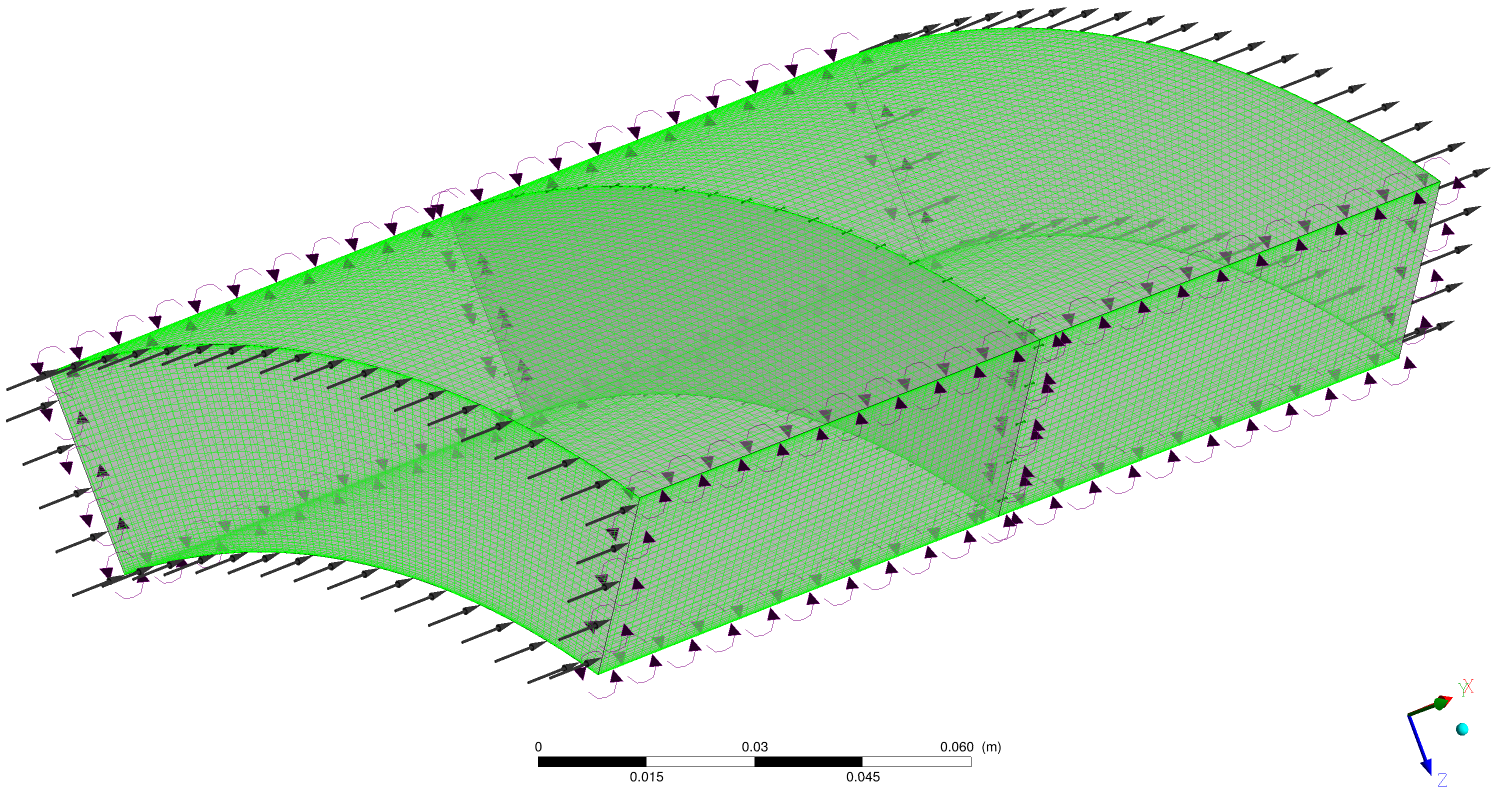
\includegraphics[width=\textwidth]{kanalmitmesh.png}
\caption{Eine dreidimensionale Ansicht der vereinfachten Aachen-Turbine mit Gitter.}
\label{fig:kanalgebiet}
\end{figure}
Die vereinfachte Turbine besteht aus einem Stator und einem Rotor. An der Vorderseite befindet sich der Einstrom, an den Seiten jeweils periodische Randbedingungen, an der Rückseite ist der Ausstrom. Die Grenzen an der Ober- und Unterseite stellen Shroud und Hub dar und werden als Wandrandbedingungen repräsentiert. Stator und Rotor sind mit einem Interface verbunden. Das Verhältnis der Abmessungen dieses Rohrausschnitts entspricht den Größenverhältnissen der Aachen-Turbine und sind der Tabelle \ref{tab:kanalabmessungen} zu entnehmen.
\begin{table}[H]
\centering
\label{tab:kanalabmessungen}
\caption{Abmessungen der vereinfachten Turbine}
\begin{tabular}{ c| c| c| c}
 $d_a$&$d_i$&$L_x$&$\alpha$\\
\hline
$300mm$&$240mm$&$160mm$&$45^\circ$\\
\end{tabular}
\end{table}
mit dem Außendurchmesser $d_a$, dem Innendurchmesser $d_i$, der Länge in Axialrichtung $L_x$ und dem Ausschnittswinkel $\alpha$.
%________________________________________________________
\subsection{Gitterstudie}
\label{subsec:kanalgitterstudie}
Nach Festlegen der Geometrie wurde ein CAD-Modell und ein Gitter mit einem $y^+ \approx 1$ erstellt. Darauf folgte eine Gitterstudie , um die Unabhängigkeit der Lösung von der Gitterdiskretition sicherzustellen. Dabei wurde das Rechengebiet auf immer feiner werdenden Gittern berechnet, bis sich die relevanten Größen nicht mehr verändert haben. In der folgenden Tabelle \ref{tab:kanalgitter} werden die Gitterparameter des Gitters gezeigt, die aus der Gitterstudie ermittelt und für die Analyse verwendet wurden. 
\begin{table}[H]
\centering
\caption{Gitterparameter des Kanals}
\begin{tabular}{ c| c| c| c| c}
$N_x$&$N_r$&$N_\phi$&Gesamtanzahl Knoten&Gesamtanzahl KV\\
\hline
48&56&79 &424704&403260\\
\end{tabular}
\label{tab:kanalgitter}
\end{table}
Dabei sind $N_x$, $N_r$ und $N_\phi$ die Anzahl an Knoten in die verschiedenen Raumrichtungen in Zylinderkoordinaten.\newline
Anschließend wurden für dieses Gitter Strömungssimulationen mit unterschiedlichen Eintrittsrandbedingungen und Veränderungen des Stator-Rotor Interfaces durchgeführt, die in dem folgendem Abschnitt beschrieben werden.

%_____________________________________________________________________________
\section{Einfluss des Stator-Rotor Interface auf den Wirkungsgrad}
\label{kanaleinfluss}
In diesem Abschnitt werden die unterschiedlichen verwendeten Eintrittsrandbedingungen näher erläutert und dann die Ergebnisse der verschiedenen Simulationen vorgestellt.
\subsection{Verwendete Eintrittsrandbedingungen}
\label{subsec:kanalrandbedingungen}
Bei dem Stator-Rotor Interface werden die Werte an den Knoten vor dem Interface nach Mittelung und Interpolation auf die Knoten nach dem Interface übertragen. Bei gleichem Gitter für Stator und Rotor können diese direkt zugeordnet werden. Deswegen wurde für einen Testfall das Gitter im Rotor verfeinert, sodass die Zuordnung der Knoten interpolativ erfolgen muss.\newline
Desweiteren wurde der Einfluss der Einstromrandbedingung in Bezug auf die Mixing Plane ermittelt. Dabei wurde eine schräge Einströmung (Abbildung \ref{fig:randbedingungen}\subref{subfig-2:randbedingungen}), eine inhomogene Temperaturverteilung mit maximaler Temperatur in Rechengebietsmitte (Abbildung \ref{fig:randbedingungen}\subref{subfig-3:randbedingungen}/\subref{subfig-4:randbedingungen}) und schließlich zusätzliche Dralleintrittsrandbedingungen mit unterschiedlicher Drallkernposition (Abbildung \ref{fig:randbedingungen}\subref{subfig-5:randbedingungen}/\subref{subfig-6:randbedingungen}) vorgegeben.
\begin{figure}[H]
\centering
%\subfigure[Feineres Gitter im Rotor]{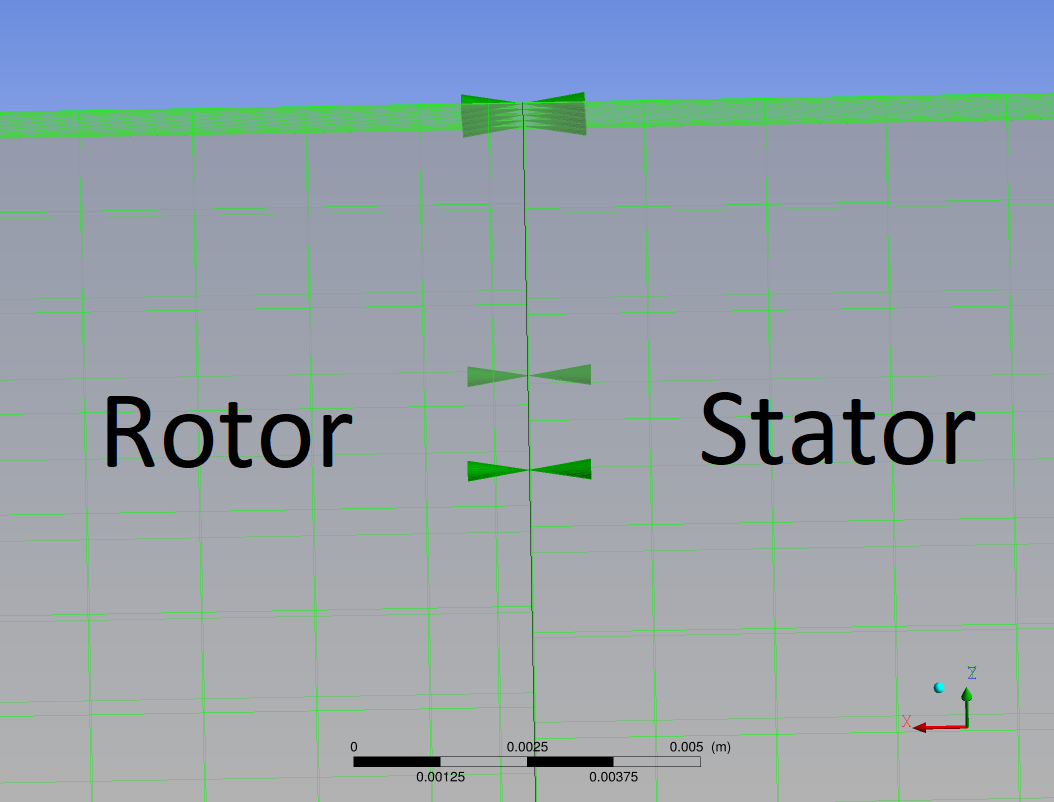
\includegraphics[width=0.45\textwidth]{bilder/feinererrotor.png}\label{subfig-1:randbedingungen}}
\subfigure[Schräger Strömungseintritt]{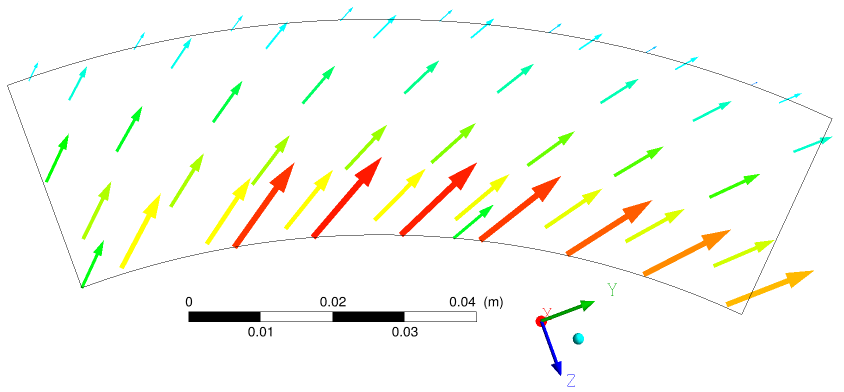
\includegraphics[width=0.8\textwidth]{schraegeStromlinien_Vector.png}\label{subfig-2:randbedingungen}}
\subfigure[Inhomogene $T_t$ (vor Interface)]{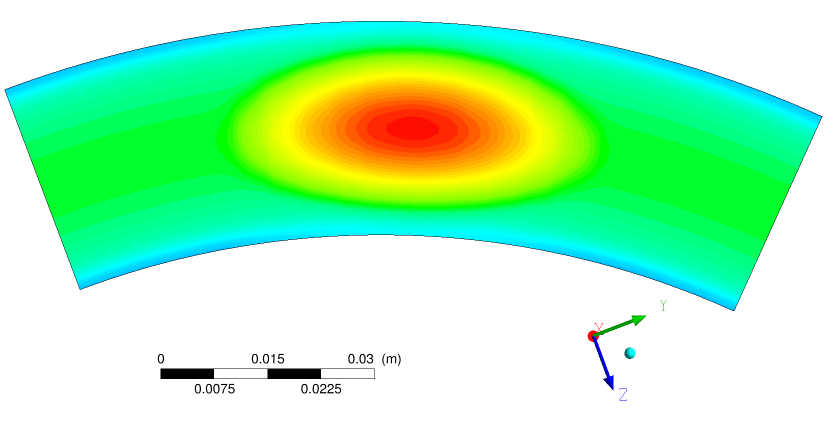
\includegraphics[width=0.45\textwidth]{TtVorMP.png}\label{subfig-3:randbedingungen}}
\subfigure[Inhomogene $T_t$ (nach Interface)]{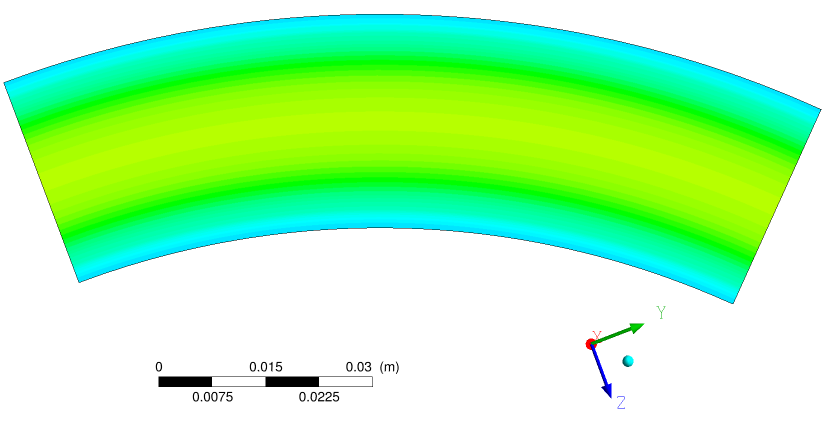
\includegraphics[width=0.45\textwidth]{TtNachMP.png}\label{subfig-4:randbedingungen}}
\subfigure[DralleintrittsRB A]{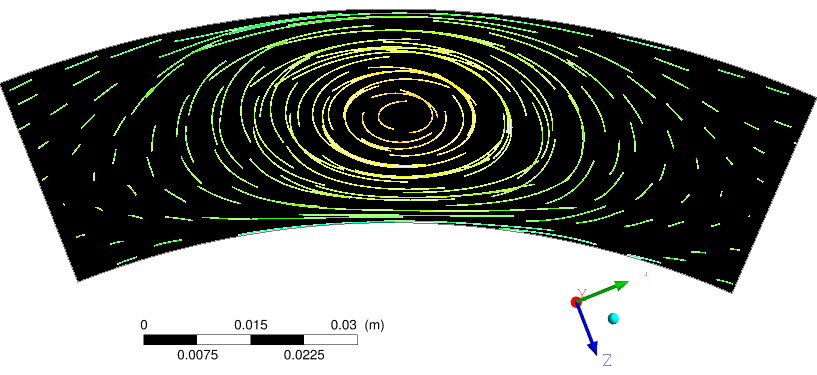
\includegraphics[width=0.45\textwidth]{drallkernA.png}\label{subfig-5:randbedingungen}}
\subfigure[DralleintrittsRB B]{\includegraphics[width=0.45\textwidth]{drallkernb.png}\label{subfig-6:randbedingungen}}
\caption{Verwendete Randbedingungen}
\label{fig:randbedingungen}
\end{figure} 
Anstatt nur stationär mit einer Mixing Plane wurde die Berechnung auch vollständig instationär mit einer Sliding Plane durchgeführt. Die Ergebnisse dieser Berechnungen werden im nächsten Abschnitt vorgestellt.
\subsection{Einfluss auf die Strömungsgrößen}
\label{subsec:kanalrandbedingungen}
Zur Untersuchung des Stator-Rotor Interface wurden die Strömungsgrößen vor und nach dem Interface miteinander verglichen, indem die Differenz nach
\begin{equation}
\label{eq:tdifferenz}
\Delta T_{t} = T_{t,2} - T_{t,1}
\end{equation}
berechnet, wobei $T_{t,1}$ die Totaltemperatur vor dem Interface und $T_{t,2}$ die Totaltemperatur nach dem Interface ist. Dabei ergibt sich folgende Tabelle \ref{tab:kanalbedingungen} mit den Strömungsgrößen Massenstrom $\dot m$, Totaldruck $p_t$ und Totaltemperatur $T_t$.
\begin{table}[H]
\centering
\caption{Einfluss der Eintrittsrandbedingungen}
\begin{tabular}{ c| c| c| c}
Einstromrandbedingung& $\Delta \dot m$ in $\frac{kg}{s}$ & $\Delta p_t$ in $Pa$ &  $\Delta T_t$ in $K$\\%&$\Delta \eta$\\
\toprule
Referenzlösung&+1,252e-05&-40,04&+0,043\\%&+0,15\%\\
feineres Gitter im Rotor&+3,755e-06&-43,81&+0,043\\%&+0,15\%\\
schräge Einströmung&-7,368e-06&-35,45&+0,026\\%&-0,04\% \\
inhomogene TemperaturRB&+1,078e-06&+10,36&+0,794\\%&+2,29\% \\
DralleintrittsRB A&-1,051e-05&-38,59&+1,764\\%&+5,45\% \\
DralleintrittsRB B&-1,312e-05&-41,83&+1,632\\%&+5,04\% \\
DralleintrittsRB C&-8,919e-06&-93,04&+1,719\\%&+5,12\% \\
DralleintrittsRB D&-1,539e-05&+2,787&+1,597\\%&+5,11\% \\
DralleintrittsRB E&+4,091e-06&-12,07&+1,576\\%&+4,99\% \\
DralleintrittsRB F&+1,729e-06&-23,83&+1,626\\%&+5,10\% \\
\midrule
Instationär&+1,873e-07&-0,604&-2,466e-04\\%&+0\% \\
\end{tabular}
\label{tab:kanalbedingungen}
\end{table}
Es ist zu sehen, dass die Massenströme vor und nach dem Stator-Rotor Interface für alle Einstrombedingungen annähernd gleich groß sind. Auch der Totaldruck unterscheidet sich um bis zu maximal $\Delta P_{t_{max}} \approx 93 Pa$ und ist somit im Vergleich zu den vorherrschenden Totaldrücken $\frac{\Delta p_t}{p_t} \approx 10^{-4}$ klein. \newline Die Totaltemperatur ändert sich bei homogenen Temperaturrandbedingungen sowohl für schräge Einströmungsrandbedingungen als auch bei feinerem Gitter im Rotor kaum ($\Delta T_t < 0,05 K$). \newline
Bei inhomogenen Temperaturrandbedingungen unterscheidet sich die Totaltemperatur vor und nach dem Interface um ungefähr $\Delta T_t \approx 0,8K$. Hier ist der Unterschied zum homogenen Temperaturfeld wesentlich größer. Insbesondere bei zusätzlichen Dralleintrittsbedingungen  ergeben sich Totaltemperaturdifferenzen von bis zu $\Delta T_t \approx 1,8K$. Bei Dralleintrittsbedingungen mit inhomogenen Randbedingungen\newline
%TO DO
Der Einfluss auf den Wirkungsgrad $\Delta \eta$ wurde durch Vergleich mit Ergebnissen der Aachen-Turbine mit gleichem Betriebspunkt abgeschätzt. 
%ZUM FAZIT
Somit ist die Berücksichtung des Einflusses der Mixing Plane für die Wirkungsgradbestimmung unerlässlich, besonders wenn inhomogene Temperaturfelder an dem Interface auftreten. Außerdem ist hier zu erwähnen, dass in diesem Testfall nur der Einfluss eines einzelnen Interfaces untersucht wurde. Bei einer Simulationen von mehreren Turbinenstufen und somit der Verwendung von mehreren Interfaces summiert sich der Fehler am Interface.

%%% Local Variables: 
%%% mode: latex
%%% TeX-master: "main"
%%% End: 


 %Dominik Keijo eingefügt
	\chapter{Auswertungstool zur Gitterstudie}
\label{cha:auswertungstool}
Für die in dieser Ausarbeitung durchgeführten Gitterstudien wurde ein Auswertungstool in Matlab erstellt. Es eignet sich für die Auswertung von Gitterstudien aus CFX-Simulationen.\\
Ziel war es, eine einfache Bedienung mit wenigen Einstellmöglichkeiten zu ermöglichen, damit dieses Tool ohne vertiefte Matlab Kenntnisse genutzt werden kann.

\begin{figure}[htbp]
	\centering
	\label{fig:auswerungbsp}
	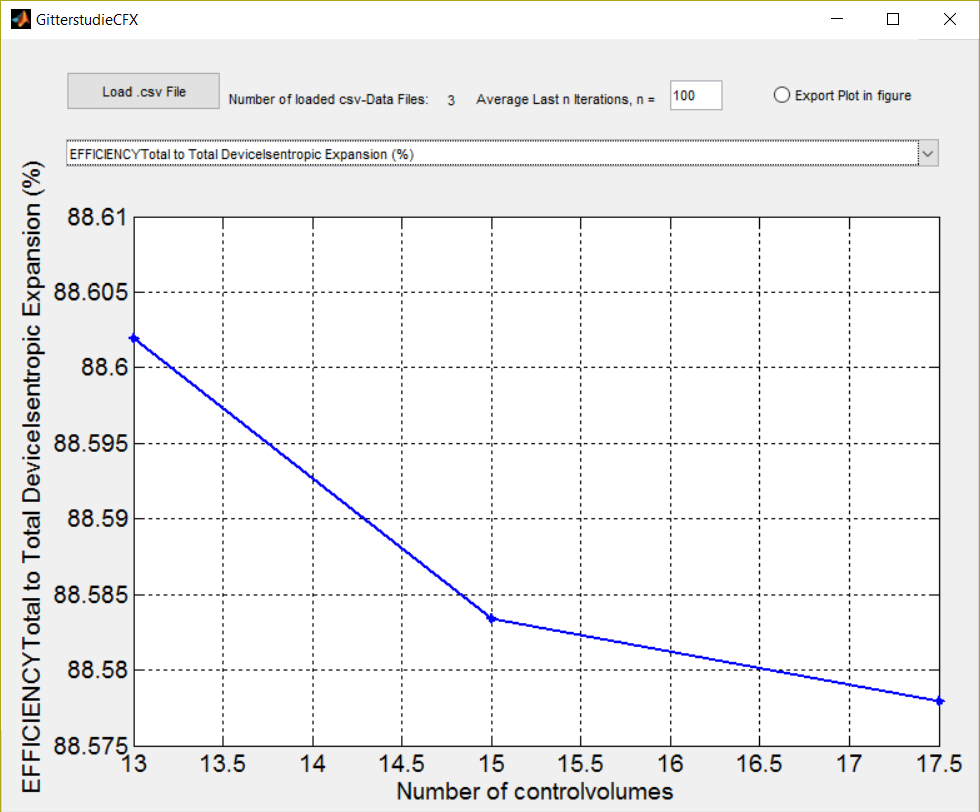
\includegraphics[width=0.8\textwidth]{auswertungstoolbsp.png}
	\caption{Auswertungstool zur Gitterstudie}
\end{figure}

\section{Funktionsumfang}
Dieses Tool stellt alle Einträge einer .csv-Datei in umgekehrter Reihenfolge da. Dadurch werden die selbst erstellten User Points im Drop-Down Menü zuerst aufgelistet. Die zu betrachtende Größe wird über der Kontrollvolumenanzahl geplottet. Dabei mittelt das Tool die letzten $n$ Iterationen einer Simulation. Durch eine Export Funktion lassen sich die Diagramme in einem separaten Fenster öffnen und können zur weiteren Verwendung in verschiedenen Formate exportiert werden.

\section{Benutzung}
Um das Tool zu verwenden, muss die Funktion \texttt{GitterstudieCFX} in Matlab ausgeführt werden. Nun können über den Button \textit{Load .csv File} csv-Dateien einzeln eingeladen werden. Diese wurden vorher mit \texttt{cfx5mondata -res filename.res -out filename.csv} in der Konsole erzeugt. In dem sich öffnenden Dialogfenster muss die Kontrollvolumenzahl, beziehungsweise  die Verfeinerungsstufe der eingelesen Datei eingegeben werden. Nach dem Einlesen kann im Drop-Down Menü die darzustellende Größe ausgewählt werden. Über den Export-Button wird das Diagramm in einem Extra-Fenster geöffnet und lässt sich in verschiedenen Formaten abspeichern.
\subsection{Wichtige Hinweise}
\lstset{language=Matlab}
\begin{description}
\item Die Dateien müssen von der gröbsten bis zur feinsten Verfeinerung in aufsteigender Reihenfolge eingeladen werden. Ansonsten springt die blaue Linie wieder zurück
\item In den Definitionen der Userpoints in CFX dürfen keine Anführungszeichen verwendet werden. Diese dienen als Trennzeichen in der .csv-Datei und führen zu zu vielen Einträgen im Drop-Down-Menü. Dadurch stimmen die dargestellten Werte nicht mehr mit dem Diagramm überein.
\item Die Schriftgröße der Achsenbeschriftung kann unter \texttt{FontSize} in den folgenden Zeilen verändert werden.
\begin{lstlisting}[frame=single]
xlabel('Number of controlvolumes','FontSize',14);
ylabel(...,'FontSize',14);
\end{lstlisting}
\item Die Schriftgröße der Achsen wird ebenfalls mit \texttt{FontSize} eingestellt.
\begin{lstlisting}[frame=single]
set(gca,'FontSize',14);
\end{lstlisting}
\item Die Linienstärke wird  mit \texttt{Linewidth} angepasst.
\begin{lstlisting}[frame=single]
plot(g(:), fPlot(:), '*-b', 'Linewidth',2);
\end{lstlisting}
\item Die Defaultwerte sorgen bereits für eine gute Lesbarkeit in Ausarbeitungen.
\item Dieses Tool mittelt standardmäßig die letzten $n=100$ Iterationen einer Simulation. Dies kann allerdings vor dem Einlesen einer Datei in dem dazugehörigen Textfeld umgestellt werden. 
\end{description}


	
	
	\listoffigures			            		             % Abbildungsverzeichnis
	\addcontentsline{toc}{chapter}{List of Figures}
	\listoftables                                    % Tabellen Verezeichnis
	\addcontentsline{toc}{chapter}{List of Tables}
	\bibliographystyle{plainnat}   			             % gibt den Stil des Literaturverzeichnises 
	\bibliography{literatur}     		             % Literaturverzeichnis
	\addcontentsline{toc}{chapter}{\bibname}         % hinzufügen ins Inhaltsverzeichnis
\end{document} 

